\begin{landscape}
{\Large\bfseries HPS-GPR v5.5.4: combining the 92 MeV excess}\par
13 September 2026 \quad | \quad Rate hypotheses, uncertainties and extracted-signal combinations
\begin{center}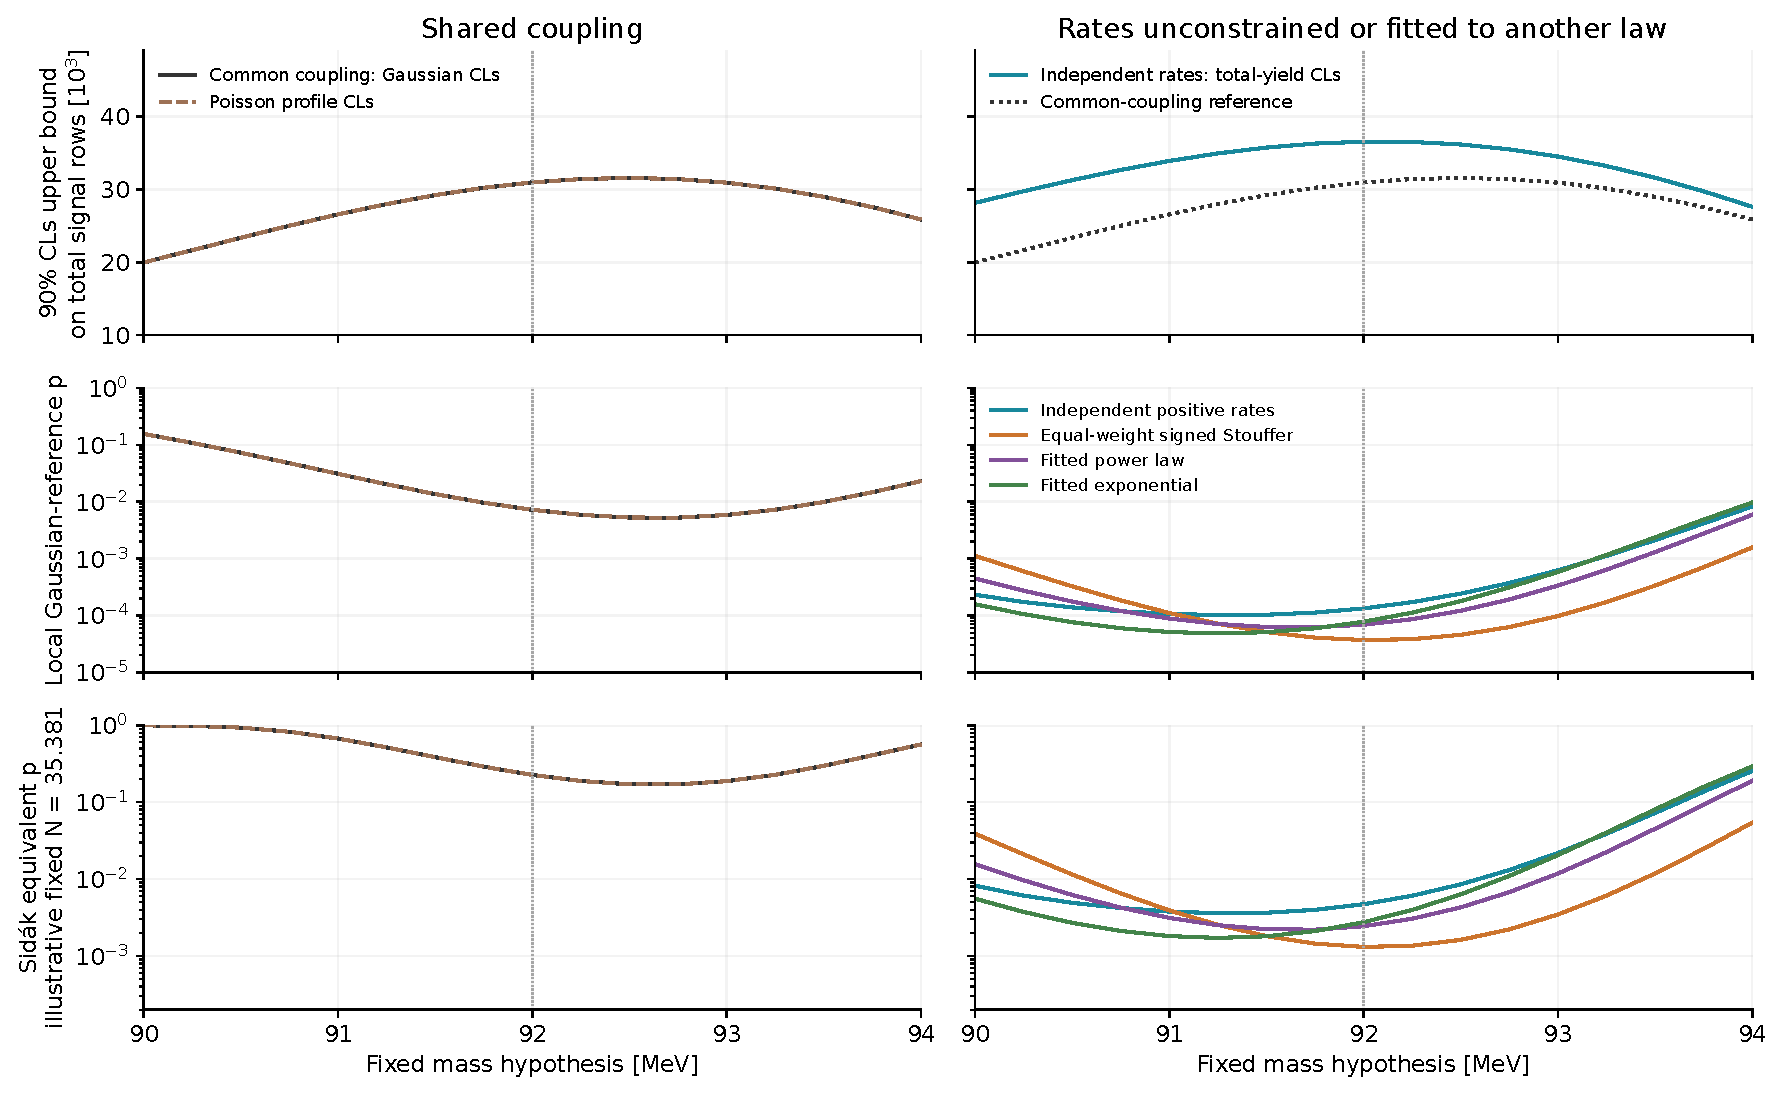
\includegraphics[height=5.2in]{../figures/coupling_vs_unconstrained_limits_pvalues.pdf}\end{center}
\captionof{figure}{The requested shared-coupling versus relaxed-rate comparison on the identical v5.5.3 experiment. Top: observed 90\% Gaussian-reference CLs bounds on the \emph{total expected signal rows in the three fit windows}; this quantity remains defined when rates are independent. Left also shows the exact Poisson-profile/asymptotic CLs result, nearly coincident with the Gaussian curve. Middle: pointwise local probabilities. Right compares distinct rate hypotheses and a signed Stouffer rule. Bottom: the same illustrative Sid\'ak mapping with inherited $N=35.381$; it is not a global calibration of these models or of this 17-point scan. All panels fix the tested mass and fully scaled widths.}
\end{landscape}
\clearpage
\begin{landscape}
\section*{Common coupling, power law and exponential with uncertainties}
\begin{center}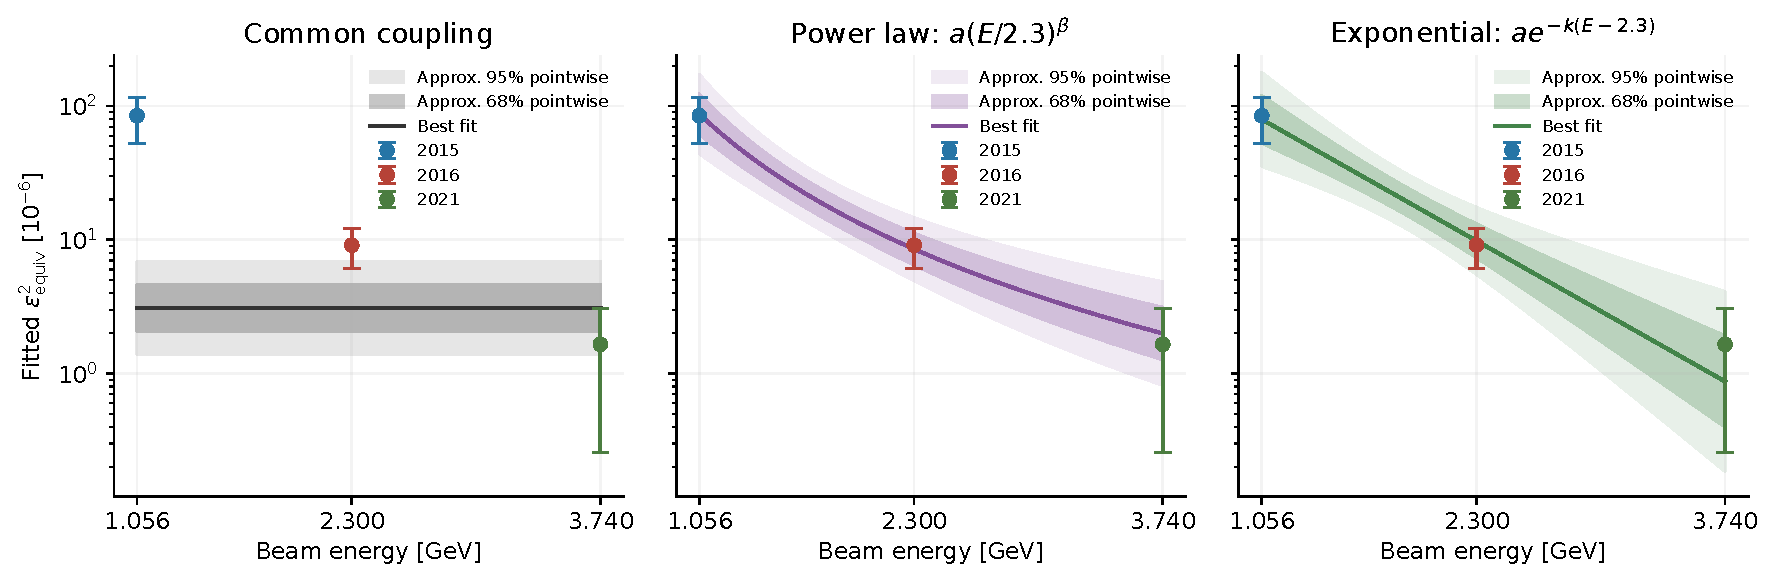
\includegraphics[width=.99\linewidth]{../figures/rate_fits_with_uncertainties.pdf}\end{center}
\captionof{figure}{An uncertainty-band version of v5.5.3 Figure 2, now separating a power law from a true decaying exponential. Points are the same independently extracted amplitudes and conditional curvature errors in all panels. Curves fit the count spectra simultaneously; shaded regions include normalization--slope covariance after profiling the GP background. Dark/light shading gives approximate 68\%/95\% \emph{pointwise log-Wald} bands at fixed 92 MeV and scaled widths. These are conditional fit uncertainties, not simultaneous bands or uncertainty on the validity of the model. The log axis makes the 2021 comparison visible.}

Write the accepted-rate normalization as $aR(E)$, with $E$ in GeV and $a$ its value at 2.30 GeV. The three fits give
\[
\begin{array}{c|c|c}
R(E)&\widehat a&\text{conditional slope interval, 68\% profile}\\\hline
1&3.102\times10^{-6}&\text{none}\\
(E/2.30)^\beta&8.516\times10^{-6}&\beta=-2.987\;[-3.517,-2.470]\\
\exp[-k(E-2.30)]&9.817\times10^{-6}&k=1.681\;[1.257,2.087]\ \mathrm{GeV}^{-1}
\end{array}
\]
The common-fit 68\% log-Wald interval on $a$ is $[2.066,4.657]\times10^{-6}$. Power and exponential fits have similar raw likelihood roots, 4.180 and 4.146. Neither residual energy law follows from a demonstrated production or detector model; the equivalent amplitudes retain the qualifications of the phenomenology discussion below. Only three beam energies constrain these two-parameter laws.
\end{landscape}
\clearpage
\begin{landscape}
\section*{Does fitting extracted signals improve the combination?}
\begin{center}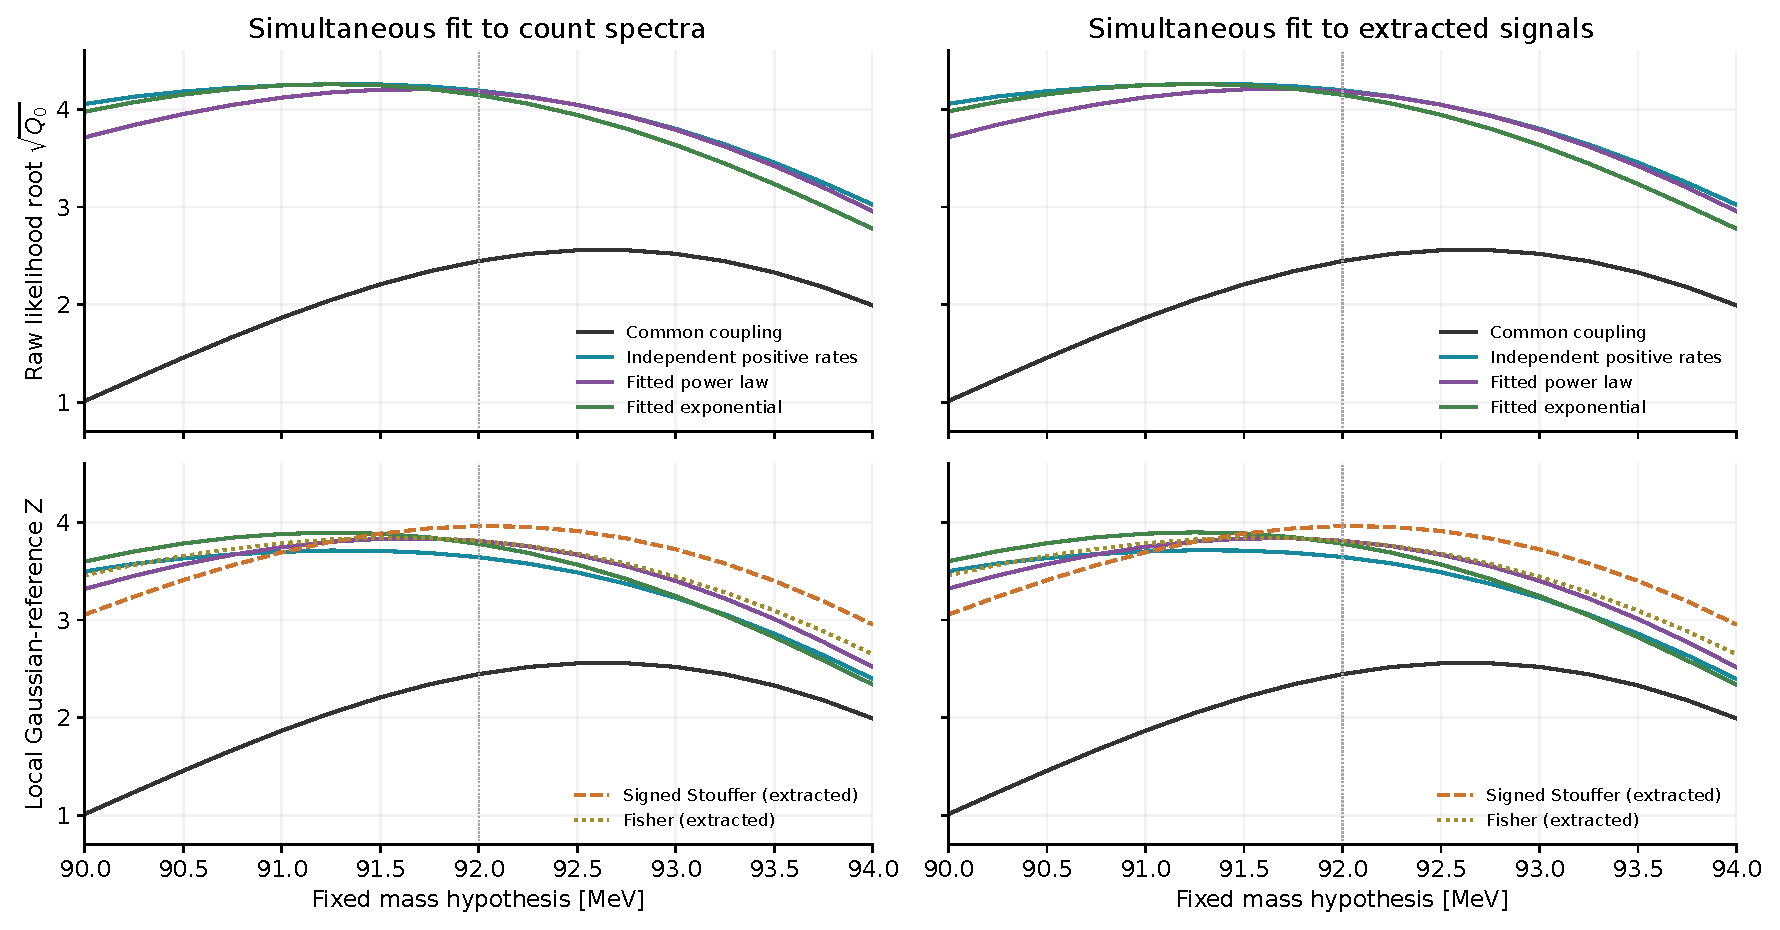
\includegraphics[height=4.25in]{../figures/spectra_vs_extracted_significance.pdf}\end{center}
\captionof{figure}{Left: simultaneous Poisson fits to the three count spectra. Right: simultaneous Gaussian fits to three signed signal estimates, retaining their uncertainties. The same mass, widths, background constraint and rate law are used across columns. Top shows raw likelihood roots; bottom shows Gaussian-reference significance with the appropriate rate-family tail. The left evaluates that reference at the exact Poisson statistic; the right uses the Gaussian statistic itself. Dashed/dotted curves are alternative Stouffer/Fisher combinations of the extracted signals, shown in both columns for comparison; they have no corresponding Poisson likelihood-root curve here.}

The two columns nearly agree. Independent experiments enter through a product likelihood, which already includes their independent information. In the fixed Gaussian experiment, the signed estimates and covariance retain all amplitude information: combining them reproduces the joint amplitude log likelihood to $5\times10^{-14}$. Fitting the extracted signals therefore checks the combination; it does not supply an additional independence factor.

Independent positive amplitudes remove the rate constraint but add freedom. Equal-weight signed Stouffer tests a chosen positive direction in standardized-score space. Selecting the strongest rule after seeing these data requires an additional correction, absent here~\cite{cowan,gross}.
\end{landscape}
\clearpage
\begin{landscape}
\section*{The local result and what its uncertainty means}
\begin{center}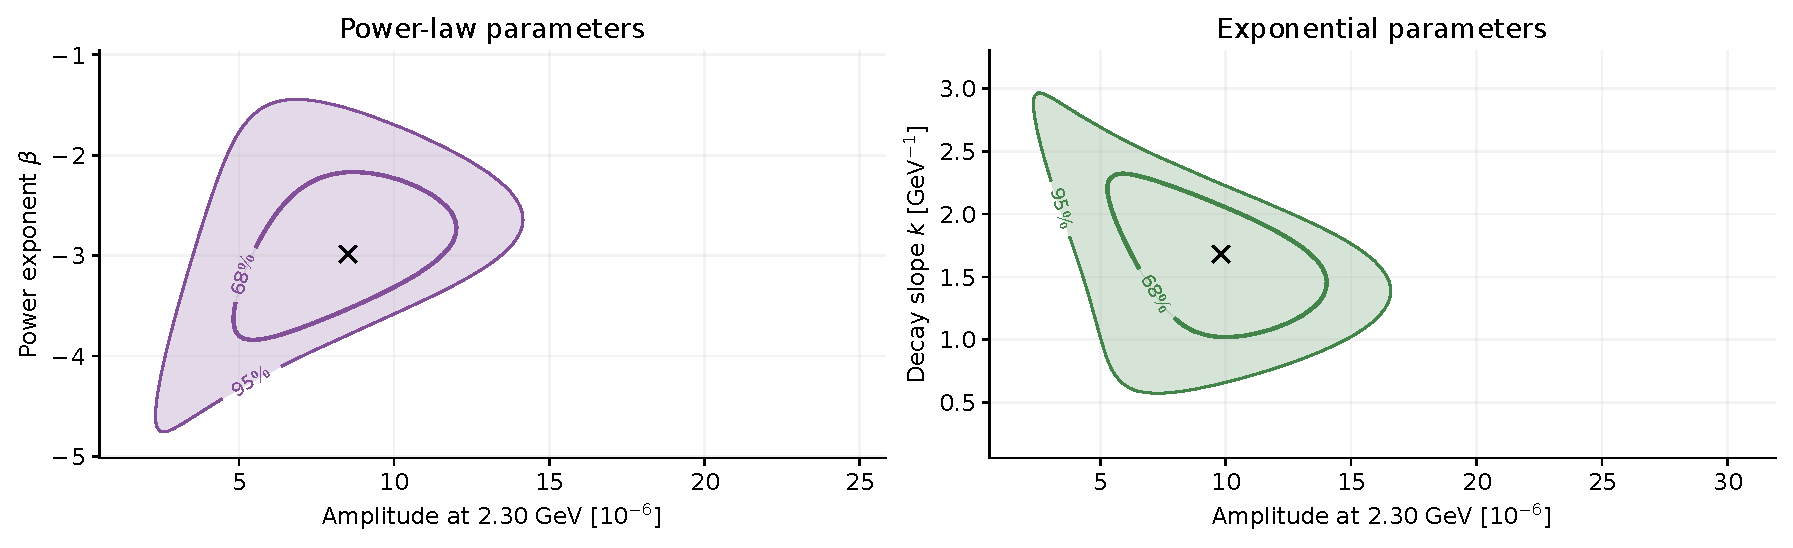
\includegraphics[height=2.35in]{../figures/rate_joint_parameter_contours.pdf}\end{center}
\captionof{figure}{Exact background-profiled likelihood contours for the two rate laws. The nominal 68\%/95\% joint levels use two-parameter asymptotic thresholds, $\Delta(2\mathrm{NLL})=2.279,5.991$; they are not coverage-calibrated regions. The correlations show why slope uncertainty must be included in the rate bands.}
\begin{center}\small\begin{tabular}{lrrr}\toprule Model or rule & $\sqrt{Q_G}$ & Local $p_G$ & $Z_G$\\\midrule
Common coupling & 2.447 & $7.21\times10^{-3}$ & 2.447\\
Independent positive amplitudes & 4.195 & $1.33\times10^{-4}$ & 3.646\\
Fitted power law & 4.182 & $6.90\times10^{-5}$ & 3.812\\
Fitted exponential & 4.148 & $7.77\times10^{-5}$ & 3.782\\
Equal-weight signed Stouffer & -- & $3.71\times10^{-5}$ & 3.962\\
Fisher of signed one-sided probabilities & -- & $6.91\times10^{-5}$ & 3.811\\
\bottomrule\end{tabular}
\end{center}
The table uses the \emph{extracted-Gaussian statistic} at fixed 92 MeV and scaled widths. For independent positive rates, $Q_G=\sum_i\max(z_i,0)^2$ has null mixture $(\chi_0^2+3\chi_1^2+3\chi_2^2+\chi_3^2)/8$. Stouffer uses $\sum_i z_i/\sqrt3$; Fisher uses $-2\sum_i\log\Phi(-z_i)$ with a $\chi_6^2$ tail. Signed scores are retained, including deficits, rather than clipping individual probabilities~\cite{heard,selfliang}. Neither rule establishes a signal in every campaign; a strong subset can drive the result.

For fitted power/exponential slopes, a deterministic three-dimensional Gaussian integral includes the slope search: integrate the $\chi_3$ radial tail over the sphere of score directions. Doubling the angular grid changes tails by at most 0.0016\%; doubling the slope grid changes them by 0.0106\%. The power-law reference at the \emph{Poisson} statistic is $Z_G=3.809$, consistent with the earlier Monte Carlo $3.815$. This calculation does not extend the earlier mass/width-search calibration.

Without a rate law, the upper-bound quantity is $T=\sum_i K_i\epsilon_i^2$. Signed Gaussian estimates give $\widehat T$ and $s_T$ for any allocation. Both opening panels use $U_{90}=\widehat T-s_T\Phi^{-1}[0.1\Phi(\widehat T/s_T)]$. At 92 MeV the bounds are 30,944 rows with common coupling and 36,523 with independent rates. These are known-covariance Gaussian-reference bounds, not detector/background-calibrated coverage. The following pages retain the v5.5.3 controls and interpretation.
\end{landscape}
\clearpage
